\documentclass[../Cours.tex]{subfiles}

\begin{document}
\chapitre{Périmètres}

\partie{Cas général}

\definition{Le périmètre d'une figure est la longueur de son contour.}

\exemple{
    \begin{center}
    \begin{tikzpicture}[scale=0.6]
        \draw[noir,gray!80!white] (0,0) grid (6,5);
        \draw[rouge, line width={0.5mm}] (1,1) -- (1,4) -- (3,4) -- (3,2) -- (4,2) -- (4,3) -- (5,3) -- (5,1) -- cycle;
        \draw[rouge, line width={0.2mm},latex-latex] (5.3,2) -- (5.3,1);
        \node[rouge, anchor=west] at (5.3,1.5) {\scriptsize{unité de longueur}};
        \node at (3,-1) {Le périmètre de cette figure est de 16 unités de longueur.};
    \end{tikzpicture}
    \end{center}
}

\propriete{Le périmètre d'un polygone est égal à la somme des longueurs de ses côtés.}

\remarque{Bien vérifier que toutes les longueurs soient exprimées dans la même unité.}

\exemple{
    \begin{center}
    \begin{tikzpicture}
        \coordinate (A) at (0,0);
        \coordinate (B) at (4,-0.8);
        \coordinate (C) at (3,2);
        \coordinate (D) at (0.5,2.5);
        \draw (0,0) node[left]{$A$} -- (4,-0.8) node[right]{$B$} -- (3,2) node[right]{$C$} -- (0.5,2.5) node[left]{$D$} -- cycle;
        \node[anchor=west] at (-5,-2) {$\curs{P}_{ABCD} = AB+BC+CD+DA=\qty{3}{\centi\metre}+\qty{2}{\centi\metre}+\qty{2.4}{\centi\metre}+\qty{1.6}{\centi\metre}$};
        \node[anchor=west] at (-5,-3) {$\curs{P}_{ABCD} = AB+BC+CD+DA=\qty{9}{\centi\metre}$};
        \node[below] at ($(A)!0.5!(B)$) {\qty{3}{\centi\metre}};
        \node[right] at ($(B)!0.5!(C)$) {\qty{2}{\centi\metre}};
        \node[above] at ($(C)!0.5!(D)$) {\qty{2.4}{\centi\metre}};
        \node[left] at ($(D)!0.5!(A)$) {\qty{1.6}{\centi\metre}};
    \end{tikzpicture}
    \end{center}
}

\partie{Formules}
\souspartie{Polygones}

\begin{center}
    \begin{tabularx}{0.9\linewidth}{|l|C|C|C|}\hline
         & Rectangle & Losange & Carré \\\hline
        Figure & \makecell{
        \begin{tikzpicture}[scale=1.2]
            \draw (0,0) rectangle (2,1);
            \node at (1,0) {||};
            \node at (1,1) {||};
            \node at (0,0.5) {*};
            \node at (2,0.5) {*};
            \draw[latex-latex] (2.3,0) -- (2.3,1) node[midway,right]{$\ell$};
            \draw[latex-latex] (0,-0.4) -- (2,-0.4) node[midway,below]{$L$};
        \end{tikzpicture}
        } & \makecell{
        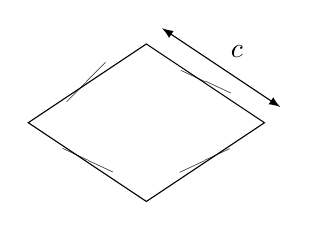
\begin{tikzpicture}
            \draw (0,0) -- (1.5,1) node[midway,rotate=45]{||} -- (3,0) node[midway,rotate=-25]{||} -- (1.5,-1) node[midway,rotate=25]{||} -- cycle node[midway,rotate=-25]{||};
            \draw[latex-latex] (1.7,1.2) -- (3.2,0.2) node[midway,above right]{$c$};
        \end{tikzpicture}
        } & \makecell{
        \begin{tikzpicture}
            \draw (-0.75,-0.75) rectangle (0.75,0.75);
            \node at (0,-0.75) {+};
            \node at (0,0.75) {+};
            \node at (-0.75,0) {+};
            \node at (0.75,0) {+};
            \draw[latex-latex] (1,-0.75) -- (1,0.75) node[midway,right]{$c$};
        \end{tikzpicture}
        } \\\hline
        Formule & $2 \times L + 2 \times \ell$ & $4 \times c$ & $4 \times c$ \\\hline
    \end{tabularx}
\end{center}

\souspartie{Cercle}

\propriete{Le périmètre d'un cercle de rayon $r$ se calcule grâce à la formule : $2 \times \pi \times r$.}

\exemple{Calculer le périmètre d'un cercle de rayon \qty{5}{\centi\metre}.
$$ \curs{P}_{\mbox{cercle}} = 2 \times \pi \times \qty{5}{\centi\metre} \approx \qty{31.4}{\centi\metre}$$
Calculer le périmètre d'un quart de cercle de rayon \qty{3}{\centi\metre}.
$$ \curs{P}_{\mbox{quart de cercle}} = \dfrac{1}{4} \times \curs{P}_{\mbox{quart de cercle}} = \dfrac{1}{4} \times 2 \times \pi \times \qty{3}{\centi\metre} \approx \qty{4.71}{\centi\metre} $$
}

\clearpage
\EXERCICES
\begin{questions}
    \exercice Calculer le périmètre de la figure ci-dessous.
    \begin{center}
        \begin{tikzpicture}
            \tikzmath{ \c=0.2; }
            \draw[fill=green!10!white] (0,0) -- ++(0,4.2) -- ++(4.6,0) -- ++(0,-2.1) node[midway,rouge]{\bfseries\textbackslash} -- ++(1.4,0) -- ++(0,-2.1) node[midway,rouge]{\bfseries\textbackslash} -- cycle; 
            \filldraw[rouge] (0,0) rectangle +(\c,\c);
            \filldraw[rouge] (0,4.2) rectangle +(\c,-\c);
            \filldraw[rouge] (4.6,4.2) rectangle +(-\c,-\c);
            \filldraw[rouge] (6,2.1) rectangle +(-\c,-\c);
            \filldraw[rouge] (6,0) rectangle +(-\c,\c);
            \draw[Latex-Latex] (-0.3,0) -- +(0,4.2) node[midway,left,anchor=east]{\qty{4.2}{\centi\metre}};
            \draw[Latex-Latex] (0,4.5) -- +(4.6,0) node[midway,above]{\qty{4.6}{\centi\metre}};
            \draw[Latex-Latex] (4.8,2.3) -- +(1.2,0) node[midway,above]{\qty{1.4}{\centi\metre}};
        \end{tikzpicture}
    \end{center}
    \exercice Comparer le périmètre d'un carré de côté \qty{42}{\milli\metre} et d'un triangle équilatéral de côté \qty{5.6}{\centi\metre}.
    \exercice Une électricienne veut fabriquer un cadre rectangulaire en métal pour installer sur un toit un nouveau panneau solaire de dimension \qty{81}{\centi\metre} sur \qty{60}{\centi\metre}. Quelle longueur de baguettes en métal doit-elle prévoir ?
    \exercice Calculer la longueur d'un côté des figures suivantes.
        \question Un carré de périmètre \qty{38}{\centi\metre}.
        \question Un triangle équilatéral de périmètre \qty{54}{\centi\metre}.
        \question Un losange de périmètre \qty{32}{\centi\metre}.

    \exercice Calculer le périmètre des figures suivantes.

    \begin{center}
        \begin{tikzpicture}[scale=0.7]
            \draw[fill=green!10!white] (0,0) -- ++(0,-5)  node[midway,rouge]{\bfseries/} -- ++(5,0)  node[midway,rouge]{\bfseries/} -- ++(0,5)  node[midway,rouge]{\bfseries/} arc (0:180:2.5);
            \draw[dashed] (0,0) -- +(5,0) node[midway,rouge]{\bfseries/};
            \draw[Latex-Latex] (-0.4,0) -- +(0,-5) node[midway,left,anchor=east]{\qty{5}{\metre}};
        \end{tikzpicture}
        \begin{tikzpicture}[scale=0.4]
            \draw[fill=orange!10!white] (0,0) arc (120:300:5) coordinate (P) arc (240:420:5) -- +(-10,0) node[midway,rouge]{\bfseries //};
            \draw[dashed] (10,0) -- (P) node[midway,rouge]{\bfseries \textbackslash\textbackslash} -- (0,0) node[midway,rouge]{\bfseries //};
            \draw[Latex-Latex] (0,0.7) -- +(10,0) node[midway,above]{\qty{10}{\metre}};
        \end{tikzpicture}
    \end{center}

    \exercice Calculer le périmètre de la figure suivante.

    \begin{center}
        \begin{tikzpicture}
            \draw[fill=green!10!white] (1.1,2) -- (0,2) node[midway,rouge]{/} -- (0,0) node[midway,rouge]{//} -- (4.2,0) -- (4.2,2) node[midway,rouge]{//} -- (3.1,2) node[midway,rouge]{/} arc (0:180:1);
            \draw[dashed] (1.1,2) -- (3.1,2) node[midway,rouge]{//};
            \draw[Latex-Latex] (0,-0.2)  -- (4.2,-0.2) node[midway,below]{\qty{42}{\centi\metre}};
            \draw[Latex-Latex] (4.5,0) -- (4.5,2) node[midway,right]{\qty{25}{\centi\metre}};
        \end{tikzpicture}  
    \end{center}

    \exercice Calculer le périmètre de la figure suivante.

    \begin{center}
        \begin{tikzpicture}
            \draw[fill=orange!10!white] (0,0) -- (0,3) node[midway,rouge]{/} node[midway,left,anchor=east]{\qty{3}{\centi\metre}} -- (8,3) -- (8,0) node[midway,rouge]{/} arc (0:-180:1) arc (0:180:3);
            \draw[dashed, Latex-Latex] (0,0) -- (6,0) node[midway,below]{\qty{6}{\centi\metre}};
            \draw[dashed, Latex-Latex] (6,0) -- (8,0) node[midway,below]{\qty{2}{\centi\metre}};
            \filldraw[rouge] (0,3) rectangle +(0.2,-0.2);
            \filldraw[rouge] (8,3) rectangle +(-0.2,-0.2);
        \end{tikzpicture}
    \end{center}

    \exercice Calculer le périmètre de la figure suivante.

    \begin{center}
        \begin{tikzpicture}
            \draw[fill=bleu!10!white] (0,0) arc(180:0:1) arc(180:0:2) arc(180:0:1) arc(0:180:4);
            \draw[dashed] (0,0) -- (8,0);
            \draw[Latex-Latex] (0,-0.4) -- (8,-0.4) node[midway,below]{\qty{8}{\centi\metre}};
            \foreach \i in {1,3,5,7} {
                \node[rouge] at (\i,0) {/};
            };
        \end{tikzpicture}
    \end{center}

    \exercice Calculer le périmètre de la figure suivante.

    \begin{center}
        \begin{tikzpicture}
            \draw[fill=rouge!10!white] (0,0) -- ++({2*cos(25},{2*sin(25)}) coordinate (a) node[midway,rouge]{//} arc(180:0:1) coordinate (c) -- ++({2*cos(25},{-2*sin(25)}) node[midway,rouge]{//} -- ++({-2*cos(25},{-2*sin(25)}) node[midway,rouge]{//} arc(0:-180:1) coordinate (b) -- ++({-2*cos(25},{2*sin(25)}) node[midway,rouge]{//};
            \draw[dashed] (a) -- ++(2,0) node[midway,rouge]{//};
            \draw[dashed] (b) -- ++(2,0) node[midway,rouge]{//};
            \draw[Latex-Latex] ($(c)+(0.3,0.2)$) -- ++({2*cos(25)},{-2*sin(25)}) node[midway,anchor=south west]{\qty{2}{\centi\metre}};
        \end{tikzpicture}
    \end{center}

    \exercice 
    \question Quel est le périmètre d'un losange de côté \qty{9}{\centi\metre} ?
    \question Quel est le périmètre d'un rectangle de longueur \qty{10}{\centi\metre} et de largeur \qty{6}{\centi\metre} ?
    \question Quel est le périmètre d'un triangle $EFG$ isocèle en $F$ tel que $EF=\qty{6}{\centi\metre}$ et $EG=\qty{4.5}{\centi\metre}$ ?

    \exercice Expliquer comment calculer le périmètre de la figure ci-dessous.
    \begin{center}
        \begin{tikzpicture}[scale=0.5]
            \draw[fill=orange!10!white] (0,0) -- ++(0,1) -- ++(1.5,0) -- ++(0,1) -- ++(1.5,0) -- ++(0,1) -- ++(3,0) -- ++(0,-1) -- ++(1.5,0) -- ++(0,-1) -- ++(1.5,0) -- ++(0,-1);
            \draw[yscale=-1,fill=orange!10!white] (0,0) -- ++(0,1) -- ++(1.5,0) -- ++(0,1) -- ++(1.5,0) -- ++(0,1) -- ++(3,0) -- ++(0,-1) -- ++(1.5,0) -- ++(0,-1) -- ++(1.5,0) -- ++(0,-1);
            \draw[Latex-Latex,rouge] (0,0) -- (9,0) node[midway,below right, rouge]{\qty{9}{\centi\metre}};
            \draw[Latex-Latex,bleu] (4.5,3) -- (4.5,-3) node[midway, above left, bleu]{\qty{6}{\centi\metre}};
        \end{tikzpicture}
    \end{center}

    \exercice 
    \question Quel est le périmètre d'un cercle de rayon \qty{4}{\centi\metre} ?
    \question Quel est le périmètre d'un cercle de diamètre \qty{12}{\centi\metre} ?

    \exercice 
    \question Quel est le diamètre d'un cercle de périmètre \qty{27}{\centi\metre} ?
    \question Quel est le rayon d'un cercle de périmètre \qty{36}{\centi\metre} ?

    \exercice Comparer les périmètres des deux figures suivantes.

    \begin{center}
        \begin{tikzpicture}
            \draw[bleu!20!white] (0,0) grid (14,6);
            \draw (1,1) rectangle +(5,4);
            \draw (8,3) -- ++(0,1) -- ++(1,0) -- ++(0,1) -- ++(1,0) -- ++(3,0) -- ++(0,-1) -- ++(1,0) -- ++(0,-1);
            \draw[yscale=-1,shift={(0,-6)}] (8,3) -- ++(0,1) -- ++(1,0) -- ++(0,1) -- ++(1,0) -- ++(3,0) -- ++(0,-1) -- ++(1,0) -- ++(0,-1);
        \end{tikzpicture}
    \end{center}

    \exercice Écrire un énoncé demandant de calculer le périmètre d'une figure dont l'expression est : $\qty{5.6}{\centi\metre} + 2 \times \qty{6.5}{\centi\metre}$.

    \exercice Tracer une figure dont l'expression ci-après permet de calculer le périmètre : $3 \times \qty{3.5}{\centi\metre} + \pi \times \qty{3.5}{\centi\metre} \div 2$    
\end{questions}

\clearpage
\CORRECTIONS

\begin{questions}
    \exercice 
    \begin{center}
        \begin{tikzpicture}
            \tikzmath{ \c=0.2; }
            \draw[fill=green!10!white] (0,0) -- ++(0,4.2) -- ++(4.6,0) -- ++(0,-2.1) node[midway,rouge]{\bfseries\textbackslash} -- ++(1.4,0) -- ++(0,-2.1) node[midway,rouge]{\bfseries\textbackslash} -- cycle; 
            \filldraw[rouge] (0,0) rectangle +(\c,\c);
            \filldraw[rouge] (0,4.2) rectangle +(\c,-\c);
            \filldraw[rouge] (4.6,4.2) rectangle +(-\c,-\c);
            \filldraw[rouge] (6,2.1) rectangle +(-\c,-\c);
            \filldraw[rouge] (6,0) rectangle +(-\c,\c);
            \draw[Latex-Latex] (-0.3,0) -- +(0,4.2) node[midway,left,anchor=east]{\qty{4.2}{\centi\metre}};
            \draw[Latex-Latex] (0,4.5) -- +(4.6,0) node[midway,above]{\qty{4.6}{\centi\metre}};
            \draw[Latex-Latex] (4.8,2.3) -- +(1.2,0) node[midway,above]{\qty{1.4}{\centi\metre}};
        \end{tikzpicture}
    \end{center}

    Pour calculer le périmètre, on va additionner les longueurs de tous les segments qui forment le pourtour de cette figure.

    \begin{align*}
        \curs{P} &= \qty{4.2}{\centi\metre} + \qty{4.6}{\centi\metre} + \qty{1.4}{\centi\metre} + \mbox{(~les deux longueurs codées par \textcolor{rouge}{\textbackslash}~)}
    \end{align*}

    Or, les deux longueurs codées par \textcolor{rouge}{\textbackslash} font la même longueur que le segment à gauche de la figure de \qty{4.2}{\centi\metre}.

    \begin{align*}
        &\curs{P} = \qty{4.2}{\centi\metre} + \qty{4.6}{\centi\metre} + \qty{1.4}{\centi\metre} + \textcolor{rouge}{\qty{4.2}{\centi\metre}} \\
        &\boxed{\curs{P} = \qty{14.4}{\centi\metre}}
    \end{align*}

    \exercice 
    \begin{align*}
        \curs{P}_{\mbox{carré}} &= 4 \times \qty{42}{\milli\metre} = \qty{168}{\milli\metre} = \qty{16.8}{\centi\metre} \\
        \curs{P}_{\mbox{triangle équilatéral}} &= 3 \times \qty{5.6}{\centi\metre} = \qty{16.8}{\centi\metre}
    \end{align*}

    Nous pouvons en conclure que les deux figures ont le même périmètre.

    \exercice 
    La forme décrite correspond à un rectangle de longueur $L = \qty{81}{\centi\metre}$ et de largeur $\ell = \qty{60}{\centi\metre}$.
    \begin{align*}
        \curs{P}_{\mbox{rectangle}} &= 2 \times L + 2 \times \ell \\
        &= 2 \times \qty{81}{\centi\metre} + 2 \times \qty{60}{\centi\metre} \\ 
        &= \qty{282}{\centi\metre} \\
        &= \boxed{\qty{2.82}{\metre}}
    \end{align*}
    Il faudra donc \qty{2.82}{\metre} pour construire ce cadre en métal.

    \exercice 
    \question 
    \begin{align*}
        \curs{P}_{\mbox{carré}} &= 4 \times \mbox{côté} = \qty{38}{\centi\metre} \\
        \mbox{côté} &= \qty{38}{\centi\metre} \div 4 = \boxed{\qty{9.5}{\centi\metre}}
    \end{align*}
    \question 
    \begin{align*}
        \curs{P}_{\mbox{triangle équilatéral}} &= 3 \times \mbox{côté} = \qty{54}{\centi\metre} \\
        \mbox{côté} &= \qty{54}{\centi\metre} \div 3 = \boxed{\qty{18}{\centi\metre}}
    \end{align*}
    \question 
    \begin{align*}
        \curs{P}_{\mbox{losange}} &= 4 \times \mbox{côté} = \qty{32}{\centi\metre} \\
        \mbox{côté} &= \qty{32}{\centi\metre} \div 4 = \boxed{\qty{8}{\centi\metre}}
    \end{align*}

    \exercice Le périmètre de la figure de gauche est composé de trois côtés d'un carré et d'un demi-cercle de rayon \qty{2.5}{\centi\metre}.

    \begin{center}
        \begin{align*}
            \curs{P} &= 3 \times \qty{5}{\metre} + \frac{1}{2} \times 2 \times \pi \times \qty{2.5}{\centi\metre} \\
            &= 15 + \pi \times \qty{2.5}{\centi\metre} \\
            &\approx \boxed{\qty{22.85}{\centi\metre}}
        \end{align*}
    \end{center}

    Le périmètre de la figure de droite est constitué de deux demi-cercles de rayon \qty{5}{\centi\metre} et d'un segment de longueur \qty{10}{\centi\metre}.

    \begin{center}
        \begin{align*}
            \curs{P} &= \qty{10}{\metre} + 2 \times \left({\color{rouge} \frac{1}{2} \times 2 \times \pi \times \qty{5}{\metre} }\right) \\
            &= \boxed{\qty{41.42}{\metre}}
        \end{align*}
    \end{center}

    \exercice 
    Le codage \textcolor{rouge}{//} correspond à \qty{25}{\centi\metre}. Le côté en haut du rectangle est composé de trois morceaux : le premier codé \textcolor{rouge}{/}, le deuxième codé \textcolor{rouge}{//} valant \qty{25}{\centi\metre} et le troisième codé comme le premier. Les trois ensembles font \qty{42}{\centi\metre}.\\
    On peut en conclure que le codage \textcolor{rouge}{/} correspond à $\dfrac{42-25}{2}=\qty{8.5}{\centi\metre}$.\\
    Le demi-cercle a pour diamètre \qty{25}{\centi\metre} donc pour rayon \qty{12.5}{\centi\metre}.
    
    \begin{align*}
        \curs{P} &= 2 \times \qty{25}{\centi\metre} + 2 \times \qty{8.5}{\centi\metre} + \qty{42}{\centi\metre} + \frac{1}{2} \times 2 \times \pi \times \qty{12.5}{\centi\metre} \\
        &\boxed{\approx \qty{148.27}{\centi\metre}}
    \end{align*}

    \exercice
    Le côté du haut mesure $6+2=\qty{8}{\centi\metre}$, ceux de gauche et de droite \qty{3}{\centi\metre}, puis la figure est également composée de deux demi-cercles, le plus grand a un diamètre de \qty{6}{\centi\metre}, donc un rayon de \qty{3}{\centi\metre}, et le plus petit a un diamètre de \qty{2}{\centi\metre}, donc un rayon de \qty{1}{\centi\metre}.

    \begin{align*}
        \curs{P} &= 2 \times \qty{3}{\centi\metre} + \qty{8}{\centi\metre} + \frac{1}{2} \times 2 \times \pi \times \qty{3}{\centi\metre} + \frac{1}{2} \times 2 \times \pi \times \qty{1}{\centi\metre} \\
        &\boxed{\approx \qty{26.57}{\centi\metre} }
    \end{align*}

    \exercice Le périmètre de cette figure est composé de 4 éléments, un grand demi-cercle de rayon \qty{4}{\centi\metre}, un moyen demi-cercle de rayon \qty{2}{\centi\metre} et deux petits demi-cercles de rayon \qty{1}{\centi\metre}.

    \begin{align*}
        \curs{P} &= \underbrace{\textcolor{vert}{\frac{1}{2} \times} 2 \times \pi \times \qty{4}{\centi\metre}}_{\mbox{grand \textcolor{vert}{demi}-cercle}} + \underbrace{ \textcolor{vert}{\frac{1}{2} \times} 2 \times \pi \times \qty{2}{\centi\metre}}_{\mbox{moyen \textcolor{vert}{demi}-cercle}} + \underbrace{ \textcolor{rouge}{2 \times} \textcolor{vert}{\frac{1}{2} \times} 2 \times \pi \times \qty{1}{\centi\metre}}_{\mbox{\textcolor{rouge}{deux} petits \textcolor{vert}{demi}-cercle}} \\
        &= 4 \times \pi + 2 \times \pi + 2 \times \pi \unit{\centi\metre} \\
        &= 8 \times \pi \unit{\centi\metre} \\ 
        &\boxed{\approx \qty{25.13}{\centi\metre}}
    \end{align*}

    \exercice Le contour de la figure est composé de 4 segments mesurant chacun \qty{2}{\centi\metre} et deux demi-cercles de rayon \qty{1}{\centi\metre}.
    \begin{align*}
        \curs{P} &= 4 \times \qty{2}{\centi\metre} + 2 \times \underbrace{\frac{1}{2} \times 2 \times \pi \times \qty{1}{\centi\metre}}_{demi-cercle} \\
        &\boxed{\approx \qty{14.28}{\centi\metre}}
    \end{align*}

    \exercice 
    \question 
    \begin{align*}
        \curs{P}_{\mbox{losange}} &= 4 \times \qty{9}{\centi\metre} \\
        &= \boxed{\qty{36}{\centi\metre}}
    \end{align*}
    \question 
    \begin{align*}
        \curs{P}_{\mbox{rectangle}} &= 2 \times \qty{10}{\centi\metre} + 2 \times \qty{6}{\centi\metre} \\ 
        &= \boxed{\qty{32}{\centi\metre}}
    \end{align*}
    \question 
    Le triangle $EFG$ est isocèle en $F$ donc $FE = FG = \qty{6}{\centi\metre}$ et $EG = \qty{4.5}{\centi\metre}$.
    \begin{align*}
        \curs{P}_{\mbox{triangle isocèle}} &= 2 \times \qty{6}{\centi\metre} + \qty{10}{\centi\metre} \\ 
        &= \boxed{\qty{22}{\centi\metre}}
    \end{align*}

    \exercice 
    Toutes les figures ci-dessous ont le même périmètre.
    \begin{center}
        \begin{tikzpicture}[scale=0.4]
            \draw[fill=orange!10!white] (0,0) -- ++(0,1) -- ++(1.5,0) -- ++(0,1) -- ++(1.5,0) -- ++(0,1) -- ++(3,0) -- ++(0,-1) -- ++(1.5,0) -- ++(0,-1) -- ++(1.5,0) -- ++(0,-1);
            \draw[yscale=-1,fill=orange!10!white] (0,0) -- ++(0,1) -- ++(1.5,0) -- ++(0,1) -- ++(1.5,0) -- ++(0,1) -- ++(3,0) -- ++(0,-1) -- ++(1.5,0) -- ++(0,-1) -- ++(1.5,0) -- ++(0,-1);
            \draw[Latex-Latex,rouge] (0,0) -- (9,0) node[midway,below right, rouge]{\qty{9}{\centi\metre}};
            \draw[Latex-Latex,bleu] (4.5,3) -- (4.5,-3) node[midway, above left, bleu]{\qty{6}{\centi\metre}};
            \draw[green,thick] (0,1) -- ++(1.5,0) -- ++(0,1);
            \draw[green,thick] (9,1) -- ++(-1.5,0) -- ++(0,1);
            \draw[green,thick] (9,-1) -- ++(-1.5,0) -- ++(0,-1);
            \draw[green,thick] (0,-1) -- ++(1.5,0) -- ++(0,-1);
        \end{tikzpicture}
        \begin{tikzpicture}[scale=0.4]
            \draw[fill=orange!10!white] (0,0) -- ++(0,1) -- ++(0,1) -- ++(1.5,0) -- ++(1.5,0) -- ++(0,1) -- ++(3,0) -- ++(0,-1) -- ++(1.5,0) -- ++(1.5,0) -- ++(0,-1) -- ++(0,-1);
            \draw[yscale=-1,fill=orange!10!white] (0,0) -- ++(0,1) -- ++(0,1) -- ++(1.5,0) -- ++(1.5,0) -- ++(0,1) -- ++(3,0) -- ++(0,-1) -- ++(1.5,0) -- ++(1.5,0) -- ++(0,-1) -- ++(0,-1);
            \draw[Latex-Latex,rouge] (0,0) -- (9,0) node[midway,below right, rouge]{\qty{9}{\centi\metre}};
            \draw[Latex-Latex,bleu] (4.5,3) -- (4.5,-3) node[midway, above left, bleu]{\qty{6}{\centi\metre}};
            \draw[green,thick] (0,1) -- ++(0,1) -- ++(1.5,0);
            \draw[green,thick] (9,1) -- ++(0,1) -- ++(-1.5,0) ;
            \draw[green,thick] (9,-1) -- ++(0,-1) -- ++(-1.5,0);
            \draw[green,thick] (0,-1) -- ++(0,-1) -- ++(1.5,0);
        \end{tikzpicture}
        \begin{tikzpicture}[scale=0.4]
            \draw[fill=orange!10!white] (0,0) -- ++(0,1) -- ++(0,1) -- ++(1.5,0) -- ++(1.5,0) -- ++(0,1) -- ++(3,0) -- ++(0,-1) -- ++(1.5,0) -- ++(1.5,0) -- ++(0,-1) -- ++(0,-1);
            \draw[yscale=-1,fill=orange!10!white] (0,0) -- ++(0,1) -- ++(0,1) -- ++(1.5,0) -- ++(1.5,0) -- ++(0,1) -- ++(3,0) -- ++(0,-1) -- ++(1.5,0) -- ++(1.5,0) -- ++(0,-1) -- ++(0,-1);
            \draw[Latex-Latex,rouge] (0,0) -- (9,0) node[midway,below right, rouge]{\qty{9}{\centi\metre}};
            \draw[Latex-Latex,bleu] (4.5,3) -- (4.5,-3) node[midway, above left, bleu]{\qty{6}{\centi\metre}};
            \draw[white,dashed,thick] (0,2) -- ++(3,0) -- ++(0,1) ;
            \draw[white,dashed,thick] (9,2) -- ++(-3,0) -- ++(0,1) ;
            \draw[white,dashed,thick] (9,-2) -- ++(-3,0) -- ++(0,-1);
            \draw[white,dashed,thick] (0,-2) -- ++(3,0) -- ++(0,-1);
        \end{tikzpicture}
        \begin{tikzpicture}[scale=0.4]
            \draw[fill=orange!10!white] (0,-3) rectangle (9,3);
            \draw[Latex-Latex,rouge] (0,0) -- (9,0) node[midway,below right, rouge]{\qty{9}{\centi\metre}};
            \draw[Latex-Latex,bleu] (4.5,3) -- (4.5,-3) node[midway, above left, bleu]{\qty{6}{\centi\metre}};
            \draw[white,dashed,thick] (0,2) -- ++(0,1) -- ++(3,0) ;
            \draw[white,dashed,thick] (9,2) -- ++(0,1) -- ++(-3,0) ;
            \draw[white,dashed,thick] (9,-2) -- ++(0,-1) -- ++(-3,0);
            \draw[white,dashed,thick] (0,-2) -- ++(0,-1) -- ++(3,0);
        \end{tikzpicture}
    \end{center}

    Cela revient à calculer donc le même périmètre qu'un rectangle.
    \begin{align*}
        \curs{P} &= 2 \times \qty{6}{\centi\metre} + 2 \times \qty{9}{\centi\metre} \\ 
        &= \boxed{\qty{30}{\centi\metre}}
    \end{align*}

    \exercice 
    \question 
    \begin{align*}
        \curs{P}_{\mbox{cercle}} &= 2 \times \pi \times \qty{4}{\centi\metre} \\ 
        &= 8 \times \pi \unit{\centi\metre} \\
        & \boxed{\approx \qty{25.23}{\centi\metre}}
    \end{align*}
    \question Si le diamètre vaut \qty{12}{\centi\metre} alors le rayon vaut \qty{6}{\centi\metre}.
    \begin{align*}
        \curs{P}_{\mbox{cercle}} &= 2 \times \pi \times \qty{6}{\centi\metre} \\ 
        &= 12 \times \pi \unit{\centi\metre} \\
        & \boxed{\approx \qty{37.70}{\centi\metre}}
    \end{align*}

    \exercice On connaît la formule $\curs{P}_{\mbox{cercle}} = 2 \times \pi \times \mbox{rayon}$. Cela signifie que si je connais le rayon, je dois le multiplier par $2 \times \pi$ pour obtenir le périmètre. \\
    Donc si je connais le périmètre, je vais l'opération dans l'autre sens et diviser par $2 \times \pi$ pour obtenir le rayon.
    \question Si le périmètre vaut \qty{27}{\centi\metre}, alors :
    \begin{align*}
        \mbox{rayon} &= \dfrac{\qty{27}{\centi\metre}}{2 \times \pi} \\ 
        & \boxed{\approx \qty{4.30}{\centi\metre}} \\
        \mbox{diamètre} &= \mbox{rayon} \times 2 \\ 
        & \boxed{\approx \qty{8.60}{\centi\metre}}
    \end{align*}
    \question Si le périmètre vaut \qty{36}{\centi\metre}, alors :
    \begin{align*}
        \mbox{rayon} &= \dfrac{\qty{36}{\centi\metre}}{2 \times \pi} \\ 
        & \boxed{\approx \qty{5.73}{\centi\metre}} \\
    \end{align*}

    \exercice Il suffit de compter les carreaux qui forment le contour des deux figures. Les deux figures ont le même périmètre : \qty{18}{carreaux}.

    \exercice Le calcul du périmètre étant $\qty{5.6}{\centi\metre} + 2 \times \qty{6.5}{\centi\metre}$, on peut comprendre que deux côtés ont pour longueur \qty{6.5}{\centi\metre} et un troisième côté qui a pour longueur \qty{5.6}{\centi\metre}.\\
    S'il y a 3 côtés, cela correspond à un triangle. Et puisque deux côtés sont égaux, il s'agit d'un triangle isocèle.\\

    << Calculer le périmètre d'un triangle isocèle tel que deux côtés mesurent \qty{6.5}{\centi\metre} et le troisième côté mesure \qty{5.6}{\centi\metre}. >>

    \clearpage
    \exercice Le périmètre de la figure étant $3 \times \qty{3.5}{\centi\metre} + \pi \times \qty{3.5}{\centi\metre} \div 2$, on comprend qu'il y a 3 côtés de même longueur \qty{3.5}{\centi\metre}.\\
    Ensuite, $\pi \times \qty{3.5}{\centi\metre} \div 2 = \dfrac{\pi \times \qty{3.5}{\centi\metre}}{2} = \dfrac{2 \times \pi \times \qty{3.5}{\centi\metre}}{2 \times 2} = \dfrac{2 \times \pi \times \qty{3.5}{\centi\metre}}{4} $. Cela correspond à un quart de cercle de rayon \qty{3.5}{\centi\metre}.

    \begin{center}
        \begin{tikzpicture}
            \draw ({3.5*cos(45)},{3.5*sin(45)}) arc(45:-45:3.5) -- (-0.94,-1.72) node[midway,rouge]{/} -- (-0.94,1.72) node[midway,rouge]{/} -- cycle node[midway,rouge]{/};
            \draw[dashed] ({3.5*cos(45)},{3.5*sin(45)}) -- ++(0,-4.95);
        \end{tikzpicture}
    \end{center}

    
    
\end{questions}


\end{document}